\documentclass{standalone}
\usepackage[margin=1in]{geometry}
\usepackage[hang,small,bf]{caption}
\usepackage{tikz}
\usepackage{braket}
\usetikzlibrary{backgrounds,shadows.blur,fit,decorations.pathreplacing,shapes}

\begin{document}
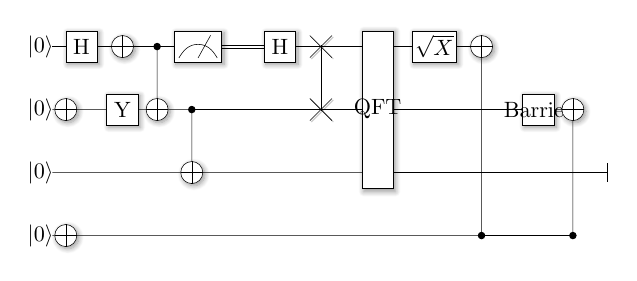
\begin{tikzpicture}[scale=0.8, transform shape]

\tikzstyle{basicshadow}=[blur shadow={shadow blur steps=8, shadow xshift=0.7pt, shadow yshift=-0.7pt, shadow scale=1.02}]\tikzstyle{basic}=[draw,fill=white,basicshadow]
\tikzstyle{operator}=[basic,minimum size=1.5em]
\tikzstyle{phase}=[fill=black,shape=circle,minimum size=0.1cm,inner sep=0pt,outer sep=0pt,draw=black]
\tikzstyle{none}=[inner sep=0pt,outer sep=-.5pt,minimum height=0.5cm+1pt]
\tikzstyle{measure}=[operator,inner sep=0pt,minimum height=0.5cm, minimum width=0.75cm]
\tikzstyle{xstyle}=[circle,basic,minimum height=0.35cm,minimum width=0.35cm,inner sep=-1pt,very thin]
\tikzset{
shadowed/.style={preaction={transform canvas={shift={(0.5pt,-0.5pt)}}, draw=gray, opacity=0.4}},
}
\tikzstyle{swapstyle}=[inner sep=-1pt, outer sep=-1pt, minimum width=0pt]
\tikzstyle{edgestyle}=[very thin]

\node[none] (line0_gate0) at (0.1,-0) {$\Ket{0}$};
\node[none] (line0_gate1) at (0.5,-0) {};
\node[none,minimum height=0.5cm,outer sep=0] (line0_gate2) at (0.75,-0) {};
\node[none] (line0_gate3) at (1.0,-0) {};
\draw[operator,edgestyle,outer sep=0.5cm] ([yshift=0.25cm]line0_gate1) rectangle ([yshift=-0.25cm]line0_gate3) node[pos=.5] {H};
\draw (line0_gate0) edge[edgestyle] (line0_gate1);
\node[xstyle] (line0_gate4) at (1.4000000000000001,-0) {};
\draw[edgestyle] (line0_gate4.north)--(line0_gate4.south);
\draw[edgestyle] (line0_gate4.west)--(line0_gate4.east);
\draw (line0_gate3) edge[edgestyle] (line0_gate4);
\node[none] (line1_gate0) at (0.1,-1) {$\Ket{0}$};
\node[xstyle] (line1_gate1) at (0.5,-1) {};
\draw[edgestyle] (line1_gate1.north)--(line1_gate1.south);
\draw[edgestyle] (line1_gate1.west)--(line1_gate1.east);
\draw (line1_gate0) edge[edgestyle] (line1_gate1);
\node[none] (line1_gate2) at (1.15,-1) {};
\node[none,minimum height=0.5cm,outer sep=0] (line1_gate3) at (1.4,-1) {};
\node[none] (line1_gate4) at (1.65,-1) {};
\draw[operator,edgestyle,outer sep=0.5cm] ([yshift=0.25cm]line1_gate2) rectangle ([yshift=-0.25cm]line1_gate4) node[pos=.5] {Y};
\draw (line1_gate1) edge[edgestyle] (line1_gate2);
\node[xstyle] (line1_gate5) at (1.9500000000000002,-1) {};
\draw[edgestyle] (line1_gate5.north)--(line1_gate5.south);
\draw[edgestyle] (line1_gate5.west)--(line1_gate5.east);
\node[phase] (line0_gate5) at (1.9500000000000002,-0) {};
\draw (line0_gate5) edge[edgestyle] (line1_gate5);
\draw (line1_gate4) edge[edgestyle] (line1_gate5);
\draw (line0_gate4) edge[edgestyle] (line0_gate5);
\node[measure,edgestyle] (line0_gate6) at (2.6000000000000005,-0) {};
\draw[edgestyle] ([yshift=-0.18cm,xshift=0.07500000000000001cm]line0_gate6.west) to [out=60,in=180] ([yshift=0.035cm]line0_gate6.center) to [out=0, in=120] ([yshift=-0.18cm,xshift=-0.07500000000000001cm]line0_gate6.east);
\draw[edgestyle] ([yshift=-0.18cm]line0_gate6.center) to ([yshift=-0.07500000000000001cm,xshift=-0.18cm]line0_gate6.north east);
\draw (line0_gate5) edge[edgestyle] (line0_gate6);
\node[none] (line0_gate7) at (3.650000000000001,-0) {};
\node[none,minimum height=0.5cm,outer sep=0] (line0_gate8) at (3.900000000000001,-0) {};
\node[none] (line0_gate9) at (4.15,-0) {};
\draw[operator,edgestyle,outer sep=0.5cm] ([yshift=0.25cm]line0_gate7) rectangle ([yshift=-0.25cm]line0_gate9) node[pos=.5] {H};
\draw ([yshift=0.02cm]line0_gate6.east) edge[edgestyle] ([yshift=0.02cm]line0_gate7.west);
\draw ([yshift=-0.02cm]line0_gate6.east) edge[edgestyle] ([yshift=-0.02cm]line0_gate7.west);
\node[none] (line2_gate0) at (0.1,-2) {$\Ket{0}$};
\node[xstyle] (line2_gate1) at (2.5000000000000004,-2) {};
\draw[edgestyle] (line2_gate1.north)--(line2_gate1.south);
\draw[edgestyle] (line2_gate1.west)--(line2_gate1.east);
\node[phase] (line1_gate6) at (2.5000000000000004,-1) {};
\draw (line1_gate6) edge[edgestyle] (line2_gate1);
\draw (line2_gate0) edge[edgestyle] (line2_gate1);
\draw (line1_gate5) edge[edgestyle] (line1_gate6);
\node[swapstyle] (line0_gate10) at (4.550000000000001,-0) {};
\draw[swapstyle,edgestyle,shadowed] ([xshift=-0.175cm,yshift=-0.175cm]line0_gate10.center)--([xshift=0.175cm,yshift=0.175cm]line0_gate10.center);
\draw[swapstyle,edgestyle,shadowed] ([xshift=-0.175cm,yshift=0.175cm]line0_gate10.center)--([xshift=0.175cm,yshift=-0.175cm]line0_gate10.center);
\node[swapstyle] (line1_gate7) at (4.550000000000001,-1) {};
\draw[swapstyle,edgestyle,shadowed] ([xshift=-0.175cm,yshift=-0.175cm]line1_gate7.center)--([xshift=0.175cm,yshift=0.175cm]line1_gate7.center);
\draw[swapstyle,edgestyle,shadowed] ([xshift=-0.175cm,yshift=0.175cm]line1_gate7.center)--([xshift=0.175cm,yshift=-0.175cm]line1_gate7.center);
\draw (line0_gate10) edge[edgestyle] (line1_gate7);
\draw (line0_gate9) edge[edgestyle] (line0_gate10);
\draw (line1_gate6) edge[edgestyle] (line1_gate7);
\node[none] (line0_gate11) at (5.2,-0) {};
\node[none,minimum height=0.5cm,outer sep=0] (line0_gate12) at (5.45,-0) {};
\node[none] (line0_gate13) at (5.7,-0) {};
\node[none] (line1_gate8) at (5.2,-1) {};
\node[none,minimum height=0.5cm,outer sep=0] (line1_gate9) at (5.45,-1) {};
\node[none] (line1_gate10) at (5.7,-1) {};
\node[none] (line2_gate2) at (5.2,-2) {};
\node[none,minimum height=0.5cm,outer sep=0] (line2_gate3) at (5.45,-2) {};
\node[none] (line2_gate4) at (5.7,-2) {};
\draw[operator,edgestyle,outer sep=0.5cm] ([yshift=0.25cm]line0_gate11) rectangle ([yshift=-0.25cm]line2_gate4) node[pos=.5] {QFT};
\draw (line0_gate10) edge[edgestyle] (line0_gate11);
\draw (line1_gate7) edge[edgestyle] (line1_gate8);
\draw (line2_gate1) edge[edgestyle] (line2_gate2);
\node[none] (line0_gate14) at (6.0,-0) {};
\node[none,minimum height=0.5cm,outer sep=0] (line0_gate15) at (6.35,-0) {};
\node[none] (line0_gate16) at (6.7,-0) {};
\draw[operator,edgestyle,outer sep=0.7cm] ([yshift=0.25cm]line0_gate14) rectangle ([yshift=-0.25cm]line0_gate16) node[pos=.5] {$\sqrt{X}$};
\draw (line0_gate13) edge[edgestyle] (line0_gate14);
\node[none] (line3_gate0) at (0.1,-3) {$\Ket{0}$};
\node[xstyle] (line3_gate1) at (0.5,-3) {};
\draw[edgestyle] (line3_gate1.north)--(line3_gate1.south);
\draw[edgestyle] (line3_gate1.west)--(line3_gate1.east);
\draw (line3_gate0) edge[edgestyle] (line3_gate1);
\node[xstyle] (line0_gate17) at (7.1,-0) {};
\draw[edgestyle] (line0_gate17.north)--(line0_gate17.south);
\draw[edgestyle] (line0_gate17.west)--(line0_gate17.east);
\node[phase] (line3_gate2) at (7.1,-3) {};
\draw (line3_gate2) edge[edgestyle] (line0_gate17);
\draw (line0_gate16) edge[edgestyle] (line0_gate17);
\draw (line3_gate1) edge[edgestyle] (line3_gate2);
\node[none] (line1_gate11) at (7.749999999999999,-1) {};
\node[none,minimum height=0.5cm,outer sep=0] (line1_gate12) at (7.999999999999999,-1) {};
\node[none] (line1_gate13) at (8.25,-1) {};
\draw[operator,edgestyle,outer sep=0.5cm] ([yshift=0.25cm]line1_gate11) rectangle ([yshift=-0.25cm]line1_gate13) node[pos=.5] {Barrier};
\draw (line1_gate10) edge[edgestyle] (line1_gate11);
\node[xstyle] (line1_gate14) at (8.549999999999999,-1) {};
\draw[edgestyle] (line1_gate14.north)--(line1_gate14.south);
\draw[edgestyle] (line1_gate14.west)--(line1_gate14.east);
\node[phase] (line3_gate3) at (8.549999999999999,-3) {};
\draw (line3_gate3) edge[edgestyle] (line1_gate14);
\draw (line1_gate13) edge[edgestyle] (line1_gate14);
\draw (line3_gate2) edge[edgestyle] (line3_gate3);
\node[none] (line2_gate5) at (9.099999999999998,-2) {};
\draw ([yshift=0.15cm]line2_gate5.center) edge [edgestyle] ([yshift=-0.15cm]line2_gate5.center);
\draw (line2_gate4) edge[edgestyle] (line2_gate5);

\end{tikzpicture}
\end{document}
